% in Terminal enter
% Rscript -e "library(knitr); knit('presentation.Rnw')"
% pdflatex presentation
% biber presentation
% pdflatex presentation
% pdflatex presentation
% 
% Einleitung
% 
% Überblick children kurz
% Wie fördern sie
% Über d verteilt
% Beide programme erklären
% Daten sammlung prozess
% Datenstruktur
% Datenaufbereitung
% 
% Summary Statistics
% 
% Mittagstisch
% Entdeckerfonds
% Subsidy
% Selfworth
% Daytodayskills
% Health variables
% 
% Regressionen
% 
% DiD-Ansatz
% 
% Grundlegende Idee – was wollen wir testen?
% Zielvariablen und warum
% Grafische evidenz 
% Resultate - Regressionstabellen
% 
% Fazit und Verbesserungsvorschläge
% 
% Gründe für fehlende effekte 
% Tipps zur datenerhebung und struktur
% partition


% when you begin a slide with a table or figure on it, always write
% \begin{frame}[fragile]
% the fragile option is important

% to make tables and figures fit, use
% scalebox = '0.75'
% or another number

% https://github.com/yihui/knitr/blob/master/inst/examples/knitr-beamer.Rnw



\documentclass{beamer}\usepackage[]{graphicx}\usepackage[]{color}
% maxwidth is the original width if it is less than linewidth
% otherwise use linewidth (to make sure the graphics do not exceed the margin)
\makeatletter
\def\maxwidth{ %
  \ifdim\Gin@nat@width>\linewidth
    \linewidth
  \else
    \Gin@nat@width
  \fi
}
\makeatother

\definecolor{fgcolor}{rgb}{0.345, 0.345, 0.345}
\newcommand{\hlnum}[1]{\textcolor[rgb]{0.686,0.059,0.569}{#1}}%
\newcommand{\hlstr}[1]{\textcolor[rgb]{0.192,0.494,0.8}{#1}}%
\newcommand{\hlcom}[1]{\textcolor[rgb]{0.678,0.584,0.686}{\textit{#1}}}%
\newcommand{\hlopt}[1]{\textcolor[rgb]{0,0,0}{#1}}%
\newcommand{\hlstd}[1]{\textcolor[rgb]{0.345,0.345,0.345}{#1}}%
\newcommand{\hlkwa}[1]{\textcolor[rgb]{0.161,0.373,0.58}{\textbf{#1}}}%
\newcommand{\hlkwb}[1]{\textcolor[rgb]{0.69,0.353,0.396}{#1}}%
\newcommand{\hlkwc}[1]{\textcolor[rgb]{0.333,0.667,0.333}{#1}}%
\newcommand{\hlkwd}[1]{\textcolor[rgb]{0.737,0.353,0.396}{\textbf{#1}}}%
\let\hlipl\hlkwb

\usepackage{framed}
\makeatletter
\newenvironment{kframe}{%
 \def\at@end@of@kframe{}%
 \ifinner\ifhmode%
  \def\at@end@of@kframe{\end{minipage}}%
  \begin{minipage}{\columnwidth}%
 \fi\fi%
 \def\FrameCommand##1{\hskip\@totalleftmargin \hskip-\fboxsep
 \colorbox{shadecolor}{##1}\hskip-\fboxsep
     % There is no \\@totalrightmargin, so:
     \hskip-\linewidth \hskip-\@totalleftmargin \hskip\columnwidth}%
 \MakeFramed {\advance\hsize-\width
   \@totalleftmargin\z@ \linewidth\hsize
   \@setminipage}}%
 {\par\unskip\endMakeFramed%
 \at@end@of@kframe}
\makeatother

\definecolor{shadecolor}{rgb}{.97, .97, .97}
\definecolor{messagecolor}{rgb}{0, 0, 0}
\definecolor{warningcolor}{rgb}{1, 0, 1}
\definecolor{errorcolor}{rgb}{1, 0, 0}
\newenvironment{knitrout}{}{} % an empty environment to be redefined in TeX

\usepackage{alltt}
% \usepackage{lmodern}
% \usepackage{lscape}
% \usepackage{graphicx}
\usepackage[utf8]{inputenc}
\usepackage[backend=biber, style=apa]{biblatex}
% \usepackage{floatrow}
\usepackage{booktabs}
\usepackage[ngerman]{babel}
\usepackage{csquotes}
% \usepackage{rotating}
% \usepackage{dcolumn}
% \usepackage{mathtools}
% \usepackage[left = 2.5cm, top = 2.5cm, right = 2.5cm, bottom = 2.0cm]{geometry}
% \usepackage[hidelinks]{hyperref}
% \usepackage{mathtools}
% \usepackage{amssymb}
% \usepackage{latexsym}
% \usepackage{eurosym}
% \usepackage{xcolor}
% \usepackage{graphicx}
% \usepackage{dcolumn}
% \usepackage{floatrow}
% \usepackage[english]{babel}
% \usepackage[utf8]{inputenc}
% \usepackage{subfigure}
% \usepackage[flushleft]{threeparttable}
% \usepackage{booktabs}
% \usepackage{adjustbox}
% \usepackage{sidecap}
% \usepackage{ifthen}
% \usepackage[backend=biber, bibstyle=apa, citestyle=authoryear]{biblatex}
% \usepackage[hidelinks]{hyperref}
% \graphicspath{{./Visuals/}}
% \setcounter{secnumdepth}{3}
% \setcounter{tocdepth}{3}
% \usepackage{url}
% \ifx\hypersetup\undefined
%   \AtBeginDocument{%
%     \hypersetup{unicode=true,pdfusetitle,
%  bookmarks=true,bookmarksnumbered=false,bookmarksopen=false,
%  breaklinks=false,pdfborder={0 0 0},pdfborderstyle={},backref=false,colorlinks=false}
%   }
% \else
%   \hypersetup{unicode=true,pdfusetitle,
%  bookmarks=true,bookmarksnumbered=false,bookmarksopen=false,
%  breaklinks=false,pdfborder={0 0 0},pdfborderstyle={},backref=false,colorlinks=false}
% \fi
% \usepackage{breakurl}
% 
% \makeatletter
%
% Fancy fit image command with optional caption copied from https://www.patrickbaylis.com/posts/2018-10-11-beamer-resizing/
% \makeatletter
% \newcommand{\fitimage}[2][\@nil]{
% 	\begin{figure}
% 		\begin{adjustbox}{width=0.9\textwidth, totalheight=\textheight-2\baselineskip-2\baselineskip,keepaspectratio}
% 			\includegraphics{#2}
% 		\end{adjustbox}
% 		\def\tmp{#1}%
% 		\ifx\tmp\@nnil
% 		\else
% 		\caption{#1}
% 		\fi
% 	\end{figure}
% }
% \makeatother
% 
% \rmfamily

\usetheme{CambridgeUS}

\setbeamerfont{subsection in toc}{size=\tiny}

\usecolortheme{crane}

\setbeamercolor{titlelike}{parent=structure, fg = black}

\addbibresource{references.bib}

%
\IfFileExists{upquote.sty}{\usepackage{upquote}}{}
\begin{document}




\title[Analyse der Survey-Daten von CHILDREN]{Analyse der Survey-Daten von CHILDREN for a better World e.V.
	}
\author[PaRE3To]{
Laura Huber\\
\and
Laura Jepsen\\
\and
Jonathan Kirschner\\
\and
Rafael Schütz\\
\and
Yannick Zurl\\
\and
Studentisches Praxisprojekt zur Empirischen Wirtschaftsforschung PaRE3To\\
\and
Ludwig-Maximilians-Universität München}
\date{3. März 2020}


\begin{frame}
	\maketitle
\end{frame}

\frame[allowframebreaks]{\frametitle{Table of Contents}
	\tableofcontents

}

\section{Einleitung}

\begin{frame}[fragile]
\frametitle{CHILDREN for a better World e.V.}
\begin{itemize}
 \item Spendenfinanzierte Kinderhilfsorganisation
 \item Finanziert Einrichtungen in ganz Deutschland
 \linebreak
 \item CHILDREN Mittagstisch: Bereitstellung von Mahlzeiten, um eine ausgewogene und gesunde Ernährung der Kinder und Jugendlichen zu fördern
 \item CHILDREN Entdeckerfonds: Durch Ausflüge und Aktivitäten wird es Kindern und Jugendlichen ermöglicht, neue Erfahrungen zu sammeln
\end{itemize}
\end{frame}


\section{Datenaufbereitung}

\begin{frame}[fragile]
\frametitle{Datenerhebung von CHILDREN}
\begin{itemize}
 \item Jährliche Umfragebögen an die Einrichtungen
 \item Beantwortung durch Mitarbeiter
 \item Verschiedene Fragen zu Mittagstisch und Entdeckerfonds
 \item Allgemeine Variablen zu den Einrichtungen (z.B. Fördersumme, Anzahl angebotener Mahlzeiten, Anzahl Aktivitäten)
 \item Abhängige Variablen zu den Kindern (z.B. Selbstwertgefühl, seltener krank)
\end{itemize}
\end{frame}

\begin{frame}[fragile]
\frametitle{Datenaufbereitung}
\begin{itemize}
 \item Zusammenfügen der Datensätze aus den verschiedenen Jahren
 \item Anpassung der Variablennamen und Hinzufügen von neuen Variablen
 \item Änderung der Datentypen von Variablen
 \item [$\Rightarrow$] Erstellung eines finalen Datensatzes
 \linebreak
 \item Datenauswertung mit dem Statistik-Programm \glqq R\grqq
 \item Versionskontrolle über \glqq Git\grqq
\end{itemize}
\end{frame}

\begin{frame}[fragile]
\frametitle{Beispiel: Datensatz}
\begin{table}[ht]
\centering
\begin{tabular}{lccccc}
  \hline
 & ID & Jahr & Anzahl der Kinder MT & Selbstwertgefühl & Ausflüge \\ 
  \hline
1 & 103 & 2014 & 30 & 3 & 4 \\ 
  2 & 103 & 2015 & 50 & 3 & 6 \\ 
  3 & 103 & 2016 & NA & 2 & 3 \\ 
  4 & 112 & 2014 & 27 & 3 & NA \\ 
  5 & 112 & 2015 & 55 & 3 & NA \\ 
  6 & 112 & 2016 & 35 & 3 & NA \\ 
   \hline
\end{tabular}
\caption{Beispielhafter Datensatz} 
\end{table}
\end{frame}

\section{Zusammenfassende Statistiken}

\subsection{Überblick: Entwickung der Anzahl der geförderten Einrichtungen}


\begin{frame}[fragile]
\frametitle{Zusammenfassende Statistiken}
% latex table generated in R 3.6.2 by xtable 1.8-4 package
<<<<<<< HEAD
% Tue Mar  3 11:15:25 2020
=======
% Tue Mar 10 17:11:31 2020
>>>>>>> 39229091d3565d1d805982cb391f2fc6d769ec5d
\begin{table}[ht]
\centering
\scalebox{0.5}{
\begin{tabular}{lccccc}
  \hline
 & Jahr & Begünstigte, Mittagstisch & Begünstigte, Entdeckerfonds & Einrichtungen, Mittagstisch & Einrichtungen, Entdeckerfonds \\ 
  \hline
1 & 2011 & 3748.0 &  & 52 &  \\ 
  2 & 2012 & 3556.0 & 2803.0 & 51 & 44 \\ 
  3 & 2013 & 4015.0 & 2823.0 & 55 & 42 \\ 
  4 & 2014 & 4685.0 & 2752.0 & 55 & 43 \\ 
  5 & 2015 & 5857.0 & 3823.0 & 55 & 49 \\ 
  6 & 2016 & 3075.0 & 3819.0 & 59 & 48 \\ 
  7 & 2017 & 4895.0 & 4150.0 & 64 & 48 \\ 
  8 & 2018 & 5102.5 & 6911.0 & 68 & 49 \\ 
   \hline
\end{tabular}
}
\caption{Zusammenfassende Statistiken} 
\label{fundamentalDynamics}
\end{table}

\end{frame}

\subsection{Entwicklung der Fördersummen über die Zeit}

\begin{frame}[fragile]
\frametitle{Umrechnung der Fördersummen: Reale Werte}
\begin{itemize}
  \item{Zur besseren Vergleichbarkeit der Fördersummen über die Zeit: Umrechnung in 2015 EUR}
  \item{Verwendung der Preisindizes des statistischen Bundesamtes}
  \item{Mittagstisch Fördersumme: Preisindex für Nahrungsmittel und alkoholfreie Getränke}
  \item{Entdeckerfonds Fördersumme: Preisindex für Freizeit, Unterhaltung und Kultur}
\end{itemize}
\end{frame}

\begin{frame}[fragile]
\frametitle{Dynamik der Fördersumme, Mittagstisch: Summe}



{\centering 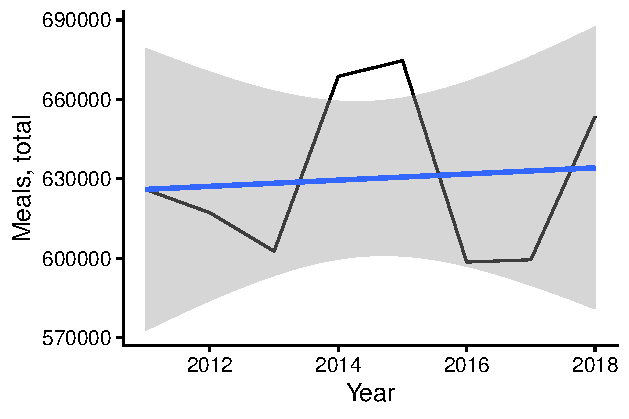
\includegraphics[width=\maxwidth]{figure/beamer-FundamentalDynamicsMealsTotal-1} 

}



\end{frame}

\begin{frame}[fragile]
\frametitle{Dynamik der Fördersumme, Mittagstisch: Median}



{\centering 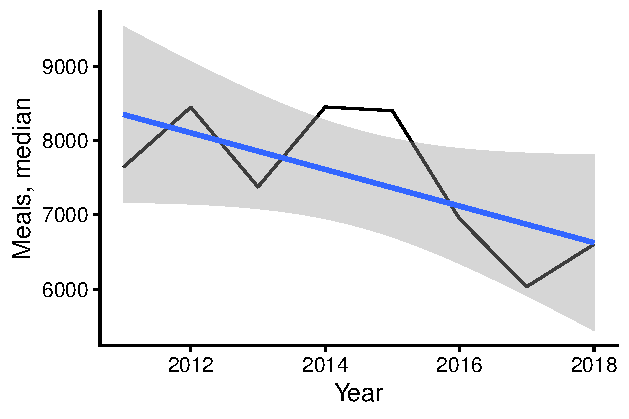
\includegraphics[width=\maxwidth]{figure/beamer-FundamentalDynamicsMealsMedian-1} 

}



\end{frame}

\begin{frame}[fragile]
\frametitle{Dynamik der Fördersumme, Mittagstisch: Median pro Begünstigter}


{\centering 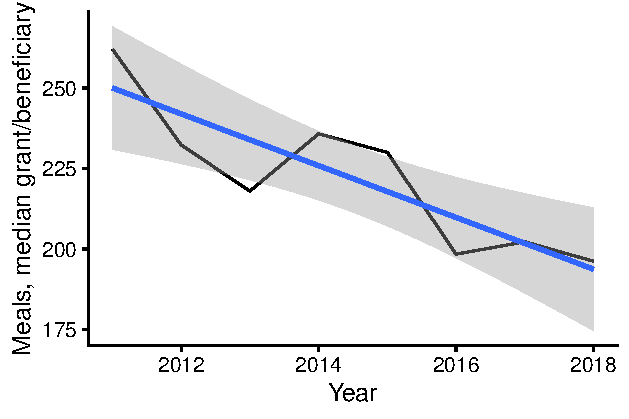
\includegraphics[width=\maxwidth]{figure/beamer-FundamentalDynamicsMealsMedianPerBene-1} 

}



\end{frame}

\begin{frame}[fragile]
\frametitle{Dynamik der Fördersumme, Entdeckerfonds: Summe}



{\centering 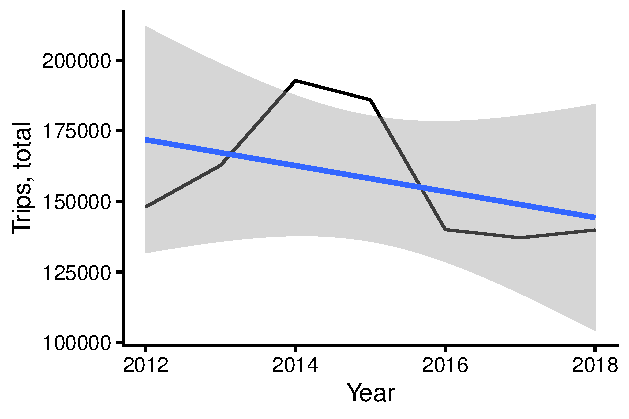
\includegraphics[width=\maxwidth]{figure/beamer-FundamentalDynamicsTripsTotal-1} 

}



\end{frame}

\begin{frame}[fragile]
\frametitle{Dynamik der Fördersumme, Entdeckerfonds: Median}



{\centering 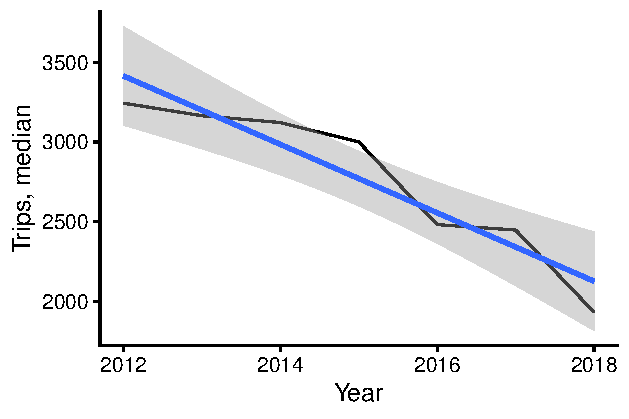
\includegraphics[width=\maxwidth]{figure/beamer-FundamentalDynamicsTripsMedian-1} 

}



\end{frame}

\begin{frame}[fragile]
\frametitle{Dynamik der Fördersumme, Entdeckerfonds: Median pro Begünstigter}


{\centering 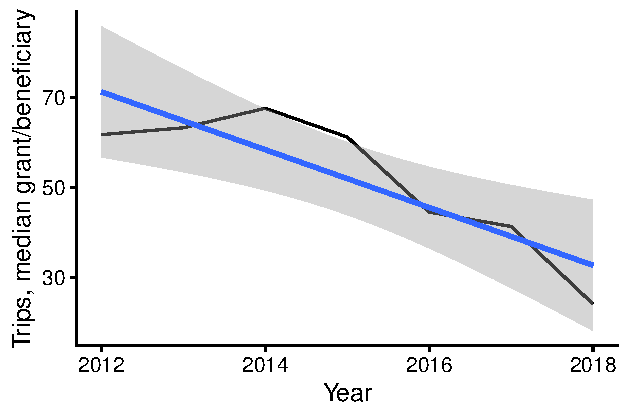
\includegraphics[width=\maxwidth]{figure/beamer-FundamentalDynamicsTripsMedianPerBene-1} 

}



\end{frame}

\subsection{Dynamiken des Selbstwertgefühls und der Alltagskompetenzen}

\begin{frame}[fragile]
\frametitle{Variable \glqq Selbstwertgefühl\grqq: Dynamik}
\begin{knitrout}\footnotesize
\definecolor{shadecolor}{rgb}{0.969, 0.969, 0.969}\color{fgcolor}

{\centering 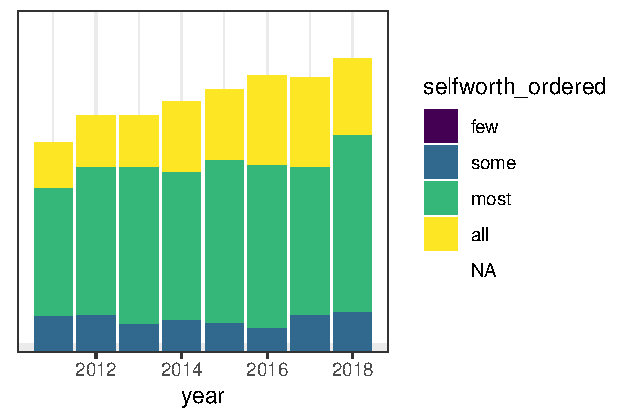
\includegraphics[width=\maxwidth]{figure/beamer-SelfworthTime-1} 

}



\end{knitrout}
\end{frame}

\begin{frame}[fragile]
\frametitle{Variable \glqq Alltagskompetenzen\grqq: Dynamik}
\begin{knitrout}\footnotesize
\definecolor{shadecolor}{rgb}{0.969, 0.969, 0.969}\color{fgcolor}

{\centering 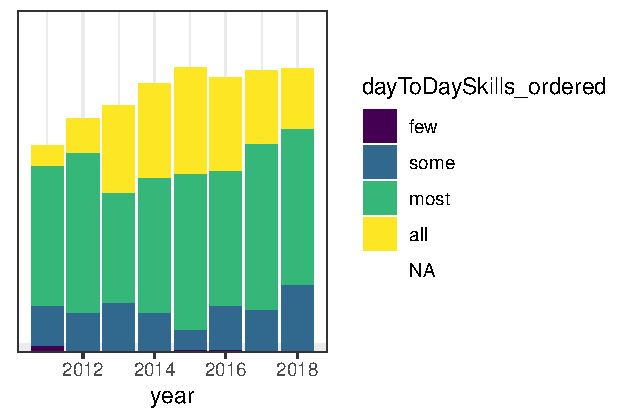
\includegraphics[width=\maxwidth]{figure/beamer-DayToDayTime-1} 

}



\end{knitrout}
\end{frame}

\subsection{Dynamiken gesundheitsrelevanter Variablen}

\begin{frame}[fragile]
\frametitle{Variable \glqq seltener krank\grqq: Dynamik}
\begin{knitrout}\footnotesize
\definecolor{shadecolor}{rgb}{0.969, 0.969, 0.969}\color{fgcolor}

{\centering 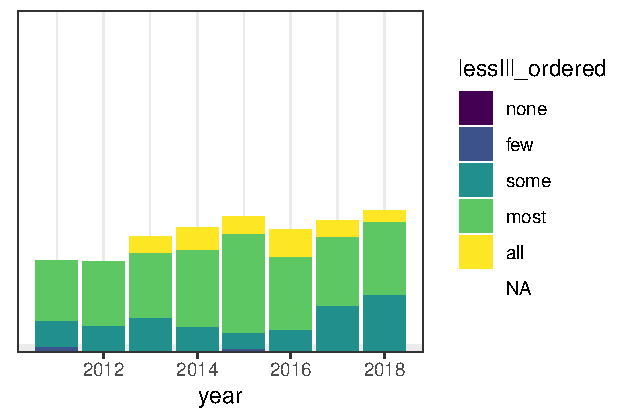
\includegraphics[width=\maxwidth]{figure/beamer-lessIllTime-1} 

}



\end{knitrout}
\end{frame}

\begin{frame}[fragile]
\frametitle{Variable \glqq erweitertes Ernährungswissen\grqq: Dynamik}
\begin{knitrout}\footnotesize
\definecolor{shadecolor}{rgb}{0.969, 0.969, 0.969}\color{fgcolor}

{\centering 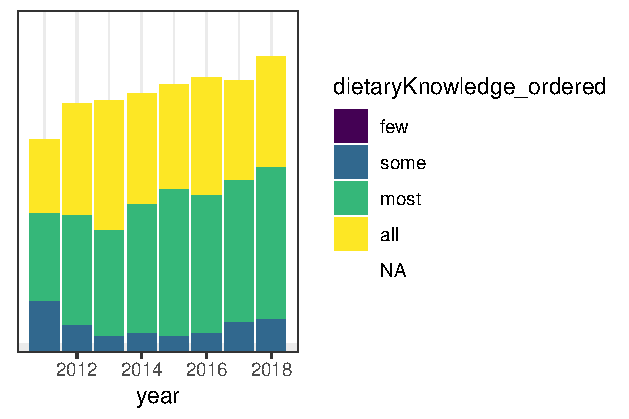
\includegraphics[width=\maxwidth]{figure/beamer-dietaryTime-1} 

}



\end{knitrout}
\end{frame}


\begin{frame}[fragile]
\frametitle{Variable \glqq Wertschätzung gesunder Ernährung\grqq: Dynamik}
\begin{knitrout}\footnotesize
\definecolor{shadecolor}{rgb}{0.969, 0.969, 0.969}\color{fgcolor}

{\centering 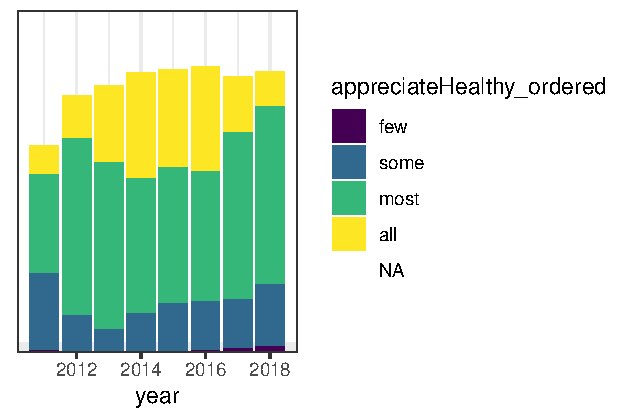
\includegraphics[width=\maxwidth]{figure/beamer-appreciateTime-1} 

}



\end{knitrout}
\end{frame}

\section{Explorative Faktoranalyse}

\begin{frame}[fragile]
\frametitle{Situation}

\begin{itemize}
 \item<1-> Viele Zielvariablen 
 \item<2-> Teilweise sehr ähnliche Zielvariablen, z.B. Begünstigte \glqq kochen mindestensts einmal im Monat in der Einrichtung\grqq und \glqq kochen mindestens einmal in der Woche in der Einrichtung\grqq
 \item<3-> Welche Variablen liegen zugrunde?
 \item<4-> Variablenreduktion zur Bestimmung möglicher Kontrollen
\end{itemize}

\end{frame}

\begin{frame}[fragile]
\frametitle{Technisches Vorgehen}

\begin{itemize}
 \item<1-> Imputierter Datensatz 
 \item<2-> Separate Faktoranalyse für jedes später zu schätzende Modell: Abhhängige Variable und Prädiktor ausgeschlossen
 \item<3-> Jede Variable als Linearkombination von wenigen Faktoren
 \item<4-> Schätzung an sich uneindeutig $\Rightarrow$ rotiere Faktoren so, dass orthogonal zueinander
\end{itemize}

\end{frame}

\begin{frame}[fragile]
\frametitle{Beispiel Faktoranalyse Mittagstisch}
% latex table generated in R 3.6.2 by xtable 1.8-4 package
<<<<<<< HEAD
% Tue Mar  3 11:15:29 2020
=======
% Tue Mar 10 17:11:42 2020
>>>>>>> 39229091d3565d1d805982cb391f2fc6d769ec5d
\begin{table}[ht]
\centering
\begin{tabular}{lcc}
  \hline
 & ML2 & ML1 \\ 
  \hline
participateMore\_scaled & 0.14 & 0.07 \\ 
  monthlyCooks\_scaled & 0.22 & 0.79 \\ 
  weeklyCooks\_scaled & 0.17 & 0.85 \\ 
  shoppers\_scaled & 0.16 & 0.55 \\ 
  easyDishes\_scaled & 0.47 & 0.44 \\ 
  dietaryKnowledge\_scaled & 0.64 & 0.20 \\ 
  appreciateHealthy\_scaled & 0.74 & 0.00 \\ 
  foodCulture\_scaled & 0.56 & 0.14 \\ 
  dayToDaySkills\_scaled & 0.57 & 0.34 \\ 
  selfworth\_scaled & 0.54 & 0.26 \\ 
  influenceHome\_scaled & 0.46 & 0.17 \\ 
   \hline
\end{tabular}
\caption{Faktoranalyse Mittagstisch ohne 'seltener krank'} 
\label{factor-analysis-example}
\end{table}



\end{frame}

\section{Partition}

\begin{frame}[fragile]
\frametitle{Alternative zu Faktoranalyse?}
\begin{itemize}
\item<1-> Neue Methode aus Biostatistik zur Dimensionalitätsreduktion: Partition \parencite{Millstein.2020}
\item<2-> Aufteilung der Menge aller Variablen in Gruppen
\item<3-> Jeder Variable wird genau eine zugrundeliegende Variable zugewiesen
\item<3-> In jeder Gruppe muss Intraklassen-Korrelationskoeffizient mindestens bestimmten, willkürlich festgelegten Wert annehmen
\item<4-> Bestimmung der Gruppen durch deterministischen Nächste-Nachbarn-Algorithmus

\end{itemize}
\end{frame}

 \begin{frame}[fragile]
 \frametitle{Partition Mittagstisch}
% latex table generated in R 3.6.2 by xtable 1.8-4 package
<<<<<<< HEAD
% Tue Mar  3 11:15:29 2020
=======
% Tue Mar 10 17:11:42 2020
>>>>>>> 39229091d3565d1d805982cb391f2fc6d769ec5d
\begin{table}[ht]
\centering
\scalebox{0.4}{
\begin{tabular}{lccc}
  \hline
 & Variable, Meals & Mapping, Meals & Information, Meals \\ 
  \hline
1 & participateMore & participateMore & 1.00 \\ 
  2 & tasksLunch & tasksLunch & 1.00 \\ 
  3 & ownIdeas & ownIdeas & 1.00 \\ 
  4 & stayLonger & stayLonger & 1.00 \\ 
  5 & dietaryKnowledge & dietaryKnowledge & 1.00 \\ 
  6 & appreciateHealthy & appreciateHealthy & 1.00 \\ 
  7 & foodCulture & foodCulture & 1.00 \\ 
  8 & lessIll & lessIll & 1.00 \\ 
  9 & betterTeamwork & betterTeamwork & 1.00 \\ 
  10 & moreRegularSchoolVisits & moreRegularSchoolVisits & 1.00 \\ 
  11 & addressProblems & addressProblems & 1.00 \\ 
  12 & reduced\_var\_1 & moreConcentrated & 0.66 \\ 
  13 & reduced\_var\_1 & moreBalanced & 0.66 \\ 
  14 & reduced\_var\_2 & monthlyCooks & 0.42 \\ 
  15 & reduced\_var\_2 & weeklyCooks & 0.42 \\ 
  16 & reduced\_var\_2 & shoppers & 0.42 \\ 
  17 & reduced\_var\_2 & easyDishes & 0.42 \\ 
  18 & reduced\_var\_3 & dayToDaySkills & 0.43 \\ 
  19 & reduced\_var\_3 & moreIndependent & 0.43 \\ 
  20 & reduced\_var\_3 & selfworth & 0.43 \\ 
  21 & reduced\_var\_3 & moreOpen & 0.43 \\ 
  22 & reduced\_var\_3 & moreConfidence & 0.43 \\ 
  23 & reduced\_var\_3 & proud & 0.43 \\ 
  24 & reduced\_var\_4 & betterReading & 0.53 \\ 
  25 & reduced\_var\_4 & betterNumbers & 0.53 \\ 
  26 & reduced\_var\_4 & betterGrades & 0.53 \\ 
  27 & reduced\_var\_5 & influenceHome & 0.41 \\ 
  28 & reduced\_var\_5 & cookAtHome & 0.41 \\ 
  29 & reduced\_var\_5 & askRecipes & 0.41 \\ 
   \hline
\end{tabular}
}
\caption{Partition der Zielvariablen, Mittagstisch} 
\label{partitionmeals}
\end{table}


 \end{frame}

\begin{frame}
\frametitle{Partition Entdeckerfonds}
% latex table generated in R 3.6.2 by xtable 1.8-4 package
<<<<<<< HEAD
% Tue Mar  3 11:15:29 2020
=======
% Tue Mar 10 17:11:42 2020
>>>>>>> 39229091d3565d1d805982cb391f2fc6d769ec5d
\begin{table}[ht]
\centering
\scalebox{0.5}{
\begin{tabular}{lccc}
  \hline
 & Variable, Trips & Mapping, Trips & Information, Trips \\ 
  \hline
1 & tripsSuggestions & tripsSuggestions & 1.00 \\ 
  2 & tripsDecisions & tripsDecisions & 1.00 \\ 
  3 & tripsOrganization & tripsOrganization & 1.00 \\ 
  4 & tripsCostCalculation & tripsCostCalculation & 1.00 \\ 
  5 & tripsBudget & tripsBudget & 1.00 \\ 
  6 & tripsMoney & tripsMoney & 1.00 \\ 
  7 & tripsReview & tripsReview & 1.00 \\ 
  8 & tripsPublicTransport & tripsPublicTransport & 1.00 \\ 
  9 & tripsMobility & tripsMobility & 1.00 \\ 
  10 & tripsAdditionalActivities & tripsAdditionalActivities & 1.00 \\ 
  11 & tripsSelfworth & tripsSelfworth & 1.00 \\ 
  12 & tripsFrustrationTolerance & tripsFrustrationTolerance & 1.00 \\ 
  13 & reduced\_var\_1 & tripsSuccess & 0.68 \\ 
  14 & reduced\_var\_1 & tripsSelfEfficacy & 0.68 \\ 
  15 & reduced\_var\_2 & tripsNewPlaces & 0.60 \\ 
  16 & reduced\_var\_2 & tripsNewCommunities & 0.60 \\ 
  17 & reduced\_var\_2 & tripsNewIdeas & 0.60 \\ 
  18 & reduced\_var\_2 & tripsSocialSkills & 0.60 \\ 
  19 & reduced\_var\_3 & tripsSpecificSkills & 0.46 \\ 
  20 & reduced\_var\_3 & tripsDayToDaySkills & 0.46 \\ 
   \hline
\end{tabular}
}
\caption{Partition der Zielvariablen, Entdeckerfonds} 
\label{partitiontrips}
\end{table}

\end{frame}




\section[Zusammenhänge]{Zusammenhänge zwischen CHILDRENs Zuschüssen, dem DGE-Kriterium und ausgewählten Variablen}

\subsection{Empirischer Ansatz}

\begin{frame}
\frametitle{Empirischer Ansatz}

\begin{equation}
\label{SimpleLinearModel}
  y_{it} = \beta_0 + \beta_1 x_{it} + \epsilon_{it}
\end{equation}

\begin{itemize}
\item Schätzung der Modelle mit OLS (Methode der kleinsten Quadrate)
\item Problem: Einrichtungen werden gleich gewichtet, unabhängig von Größe
\item Lösung: Modellschätzung mit WLS (Gewichtete kleinste Quadrate)
\item [$\Rightarrow$] Gewichte: Anzahl der regelmäßigen Teilnehmer am Mittagstisch und im Entdeckerfonds
\end{itemize}

\end{frame}

\begin{frame}[fragile]
\frametitle{Variante: Imputieren fehlender Werte}
\begin{itemize}
\item Problem: Viele Einrichtungen beantworten nicht alle Fragen
\begin{itemize}
\item Lösung: Erstellung eines seperaten Datensatzes in welchem fehlende Werte imputiert werden
\item [$\Rightarrow$] Imputieren der Daten mit einrichtungs-spezifischem linearen Trend
\end{itemize}
\item Vergleich von Regressionen mit den Daten des originalen Datenatzes mit den imputierten Daten
\end{itemize}
\end{frame}


\begin{frame}[fragile]
\frametitle{Variante: Ausschließen von Ausreißern}
\begin{itemize}
\item Problem: CHILDREN fördert Einrichtungen mit sehr vielen und sehr wenigen ausgegebenen Essen und unternommenen Ausflügen
\item Lösung: Datensätze ohne Ausreißer
\item Mittagstisch: Ausreißer bei Anzahl von Essen
\item Entdeckerfonds: Ausreißer bei Anzahl von Ausflügen
\item Definition eines Ausreißers:
\begin{itemize}
\item Werte, die 1,5 Interquantilsabstände unter dem 25\%-Perzentil liegen
\item Werte, die 1,5 Interqauntilsabstände über dem 75\%-Perzentil liegen
\end{itemize}
\end{itemize}
\end{frame}

\subsection{Assoziationen zwischen Fördersumme und ausgewählten Variablen}

\begin{frame}[fragile]
\frametitle{Assoziationen zwischen:}
\begin{itemize}
\item Fördersumme für Mittagstisch (in 2015 EUR) und Anzahl ausgegebener Essen
\item Fördersumme für Entdeckerfonds (in 2015 EUR) und Anzahl unternommener Ausflüge
\item Sowohl für Mittagstisch als auch für Entdeckerfonds:
\begin{itemize}
\item Fördersumme pro Begünstigter (in 2015 EUR) und standardisierter Anteil der Begünstigten mit gestiegenen Selbstwertgefühl
\item Fördersumme pro Begünstigter (in 2015 EUR) und standardisierter Anteil der Begünstigten mit erweiterten Alltagskompetenzen
\end{itemize}
\end{itemize}
\end{frame}


\begin{frame}[fragile]
\frametitle{Anzahl Mahlzeiten und Fördersumme}


\begin{table}
\caption{Zusammenhang zwischen Anzahl der Mahlzeiten und realer Fördersumme}
\begin{center}
\scalebox{0.5}{
\begin{tabular}{l c c c c c }
\toprule
 & (1) & (2) & (3) & (4) & (5) \\
\midrule
(Intercept)     & $-12089.14^{*}$ & $-1814.16$     & $3535.39^{***}$ & $3107.70^{***}$ & $-12250.60^{**}$ \\
                & $(5192.86)$     & $(1765.93)$    & $(498.99)$      & $(508.94)$      & $(4524.09)$      \\
realSubsidy     & $2.61^{***}$    & $0.50^{**}$    & $0.29^{***}$    & $0.25^{***}$    & $2.72^{***}$     \\
                & $(0.57)$        & $(0.18)$       & $(0.05)$        & $(0.05)$        & $(0.51)$         \\
eatersPerMealNo &                 & $172.83^{***}$ &                 & $19.00^{*}$     &                  \\
                &                 & $(14.92)$      &                 & $(8.45)$        &                  \\
\midrule
R$^2$           & 0.43            & 0.73           & 0.13            & 0.21            & 0.45             \\
Adj. R$^2$      & 0.43            & 0.73           & 0.12            & 0.20            & 0.45             \\
Num. obs.       & 329             & 329            & 250             & 250             & 440              \\
RMSE            & 39992.79        & 27390.90       & 3629.72         & 3463.66         & 39601.41         \\
\bottomrule
\multicolumn{6}{l}{\scriptsize{\parbox{\linewidth}
{\vspace{2pt} Abhängige Variable: Anzahl der Mahlzeiten \\ realSubsidy: Fördersumme für Mittagstisch (EUR von 2015)\\ eatersPerMeal: Anzahl der durch Mittagtisch Begünstigten \\ Modell (1): einfaches lineares Modell, geschätzt mit Methode der kleinsten Quadrate \\ Modell (2): ursprünglicher Datensatz, lineares Modell mit Kontrollen, geschätzt mit Methode der kleinsten Quadrate \\ Modell (3): Datensatz ohne Ausreißer, einfaches lineares Modell, geschätzt mit Methode der kleinsten Quadrate \\ Modell (4): Datensatz ohne Ausreißer, lineares Modell mit Kontrollen, geschätzt mit Methode der kleinesten Quadrate \\ Modell (5): Datensatz mit durch lineare Interpolation pro Einrichtung imputierten Daten, einfaches lineare Modell, geschätzt mit Methode der kleinsten Quadrate  \\ Alle Standardfehler sind robust. $^{***}p<0.001$, $^{**}p<0.01$, $^*p<0.05$.}}}
\end{tabular}
}
\label{GrantsRegressionsLunch}
\end{center}
\end{table}

\end{frame}

\begin{frame}[fragile]
\frametitle{Anzahl Ausflüge und Fördersumme}

\begin{table}
\caption{Zusammenhang zwischen Anzahl Ausflüge und Fördersumme}
\begin{center}
\scalebox{0.7}{
\begin{tabular}{l c c c c c }
\toprule
 & (1) & (2) & (3) & (4) & (5) \\
\midrule
(Intercept)      & $3.7049^{***}$ & $3.4394^{***}$ & $2.6236^{***}$ & $2.3660^{***}$ & $3.6237^{***}$ \\
                 & $(0.3313)$     & $(0.3359)$     & $(0.2300)$     & $(0.2609)$     & $(0.3253)$     \\
realTripsSubsidy & $0.0002^{*}$   & $0.0001$       & $0.0003^{***}$ & $0.0003^{***}$ & $0.0002^{*}$   \\
                 & $(0.0001)$     & $(0.0001)$     & $(0.0001)$     & $(0.0001)$     & $(0.0001)$     \\
tripsKidsNo      &                & $0.0059$       &                & $0.0043$       &                \\
                 &                & $(0.0032)$     &                & $(0.0027)$     &                \\
\midrule
R$^2$            & 0.0474         & 0.0729         & 0.0880         & 0.1241         & 0.0504         \\
Adj. R$^2$       & 0.0444         & 0.0671         & 0.0844         & 0.1172         & 0.0476         \\
Num. obs.        & 322            & 319            & 257            & 256            & 334            \\
RMSE             & 2.9565         & 2.8967         & 1.6981         & 1.6579         & 2.9310         \\
\bottomrule
\multicolumn{6}{l}{\scriptsize{\parbox{\linewidth}
{\vspace{2pt} Dependent variable: number of trips \\ realTripsSubsidy: subsidy for Trips program in 2015 EUR \\ tripsKidsNo: number of beneficiaries of Trips program \\ Model (1): original data set, simple linear model, estimated with OLS \\ Model (2): original data set, linear model with controls, estimated with OLS \\ Model (3): data set without outliers, simple linear model, esmitaed with OLS \\ Model (4): data set without outliers, linear model with controls, estimated with OLS \\ Model (5): imputed data set, simple linear model, estimated with OLS \\ All regressions are estimated with robust standard errors $^{***}p<0.001$, $^{**}p<0.01$, $^*p<0.05$.}}}
\end{tabular}
}
\label{GrantsRegressionsTrips}
\end{center}
\end{table}

\end{frame}

\begin{frame}[fragile]
\frametitle{Selbstwertgefühl und Fördersumme pro Begünstigter}


\begin{table}
\caption{Zusammenhang zwischen Selbstwertgefühl und Fördersumme pro Begünstigtem}
\begin{center}
\scalebox{0.4}{
\begin{tabular}{l c c c c c }
\hline
 & (1) & (2) & (3) & (4) & (5) \\
\hline
(Intercept)                    & $0.08$   & $0.12$   & $0.09$   & $0.12$   & $0.23^{*}$   \\
                               & $(0.09)$ & $(0.12)$ & $(0.09)$ & $(0.11)$ & $(0.11)$     \\
realSubsidyPerBeneficiary      & $-0.00$  &          & $-0.00$  &          & $-0.00$      \\
                               & $(0.00)$ &          & $(0.00)$ &          & $(0.00)$     \\
realTripsSubsidyPerBeneficiary &          & $-0.00$  &          & $-0.00$  &              \\
                               &          & $(0.00)$ &          & $(0.00)$ &              \\
ML1                            &          &          &          &          & $0.24^{***}$ \\
                               &          &          &          &          & $(0.06)$     \\
ML2                            &          &          &          &          & $0.37^{***}$ \\
                               &          &          &          &          & $(0.05)$     \\
ML3                            &          &          &          &          & $0.15^{***}$ \\
                               &          &          &          &          & $(0.04)$     \\
\hline
R$^2$                          & 0.00     & 0.01     & 0.00     & 0.01     & 0.30         \\
Adj. R$^2$                     & 0.00     & 0.01     & 0.00     & 0.01     & 0.28         \\
Num. obs.                      & 428      & 184      & 430      & 187      & 161          \\
RMSE                           & 1.00     & 1.00     & 1.00     & 1.00     & 0.79         \\
\hline
\multicolumn{6}{l}{\scriptsize{\parbox{\linewidth}
{\vspace{2pt} realSubsidyPerBeneficiary: subsidy per beneficiary of Meals program in 2015 EUR \\ realTripsSubsidyPerBeneficiary: subsidy per beneficiary of Trips program in 2015 EUR \\Model (1): dependent variable: share of beneficiaries with improved self-worth in the Lunch program, original data set, simple linear model, estimated with OLS \\ Model (2): dependent variable: share of beneficiaries with improved self-worth in the Trips program, original data set, simple linear model, estimated with OLS \\ Model (3): dependent variable: share of beneficiaries with improved self-worth in the Lunch program, imputed data set, simple linear model, estimated with OLS \\ Model (4): dependent variable: share of beneficiaries with improved self-worth in the Trips program, imputed data set, simple linear model, estimated with OLS \\ Model (5): dependent variable: share of beneficiaries with improved self-worth in the Lunch program, imputed data set, linear model with extracted factor scores as controls, estimated with OLS \\ All regressions are estimated with robust standard errors $^{***}p<0.001$, $^{**}p<0.01$, $^*p<0.05$.}}}
\end{tabular}
}
\label{SelfworthRegressions}
\end{center}
\end{table}


\end{frame}

\begin{frame}[fragile]
\frametitle{Alltagskompetenzen und Fördersumme pro Begünstigter}


\begin{table}
\caption{Zusammenhang zwischen Alltagskompetenzen und Fördersumme pro Begünstigtem}
\begin{center}
\scalebox{0.4}{
\begin{tabular}{l c c c c c c }
\hline
 & (1) & (2) & (3) & (4) & (5) & (6) \\
\hline
(Intercept)                    & $0.15$   & $0.13$   & $0.14$   & $0.11$   & $0.28^{*}$   & $0.08$       \\
                               & $(0.09)$ & $(0.10)$ & $(0.09)$ & $(0.10)$ & $(0.11)$     & $(0.09)$     \\
realSubsidyPerBeneficiary      & $-0.00$  &          & $-0.00$  &          & $-0.00$      &              \\
                               & $(0.00)$ &          & $(0.00)$ &          & $(0.00)$     &              \\
realTripsSubsidyPerBeneficiary &          & $-0.00$  &          & $-0.00$  &              & $-0.00$      \\
                               &          & $(0.00)$ &          & $(0.00)$ &              & $(0.00)$     \\
ML1                            &          &          &          &          & $0.31^{***}$ & $0.03$       \\
                               &          &          &          &          & $(0.06)$     & $(0.07)$     \\
ML2                            &          &          &          &          & $0.40^{***}$ & $0.16^{*}$   \\
                               &          &          &          &          & $(0.06)$     & $(0.07)$     \\
ML3                            &          &          &          &          & $0.16^{**}$  & $0.19^{**}$  \\
                               &          &          &          &          & $(0.05)$     & $(0.06)$     \\
ML4                            &          &          &          &          &              & $0.49^{***}$ \\
                               &          &          &          &          &              & $(0.06)$     \\
\hline
R$^2$                          & 0.01     & 0.01     & 0.01     & 0.01     & 0.37         & 0.37         \\
Adj. R$^2$                     & 0.01     & 0.01     & 0.01     & 0.01     & 0.36         & 0.35         \\
Num. obs.                      & 426      & 177      & 429      & 181      & 161          & 169          \\
RMSE                           & 1.00     & 0.98     & 1.00     & 0.99     & 0.78         & 0.80         \\
\hline
\multicolumn{7}{l}{\scriptsize{\parbox{\linewidth}
{\vspace{2pt} realSubsidyPerBeneficiary: subsidy per beneficiary of Meals program in 2015 EUR \\ realTripsSubsidyPerBeneficiary: subsidy per beneficiary of Trips program in 2015 EUR \\ Model (1): dependent variable: share of beneficiaries with with broadened everyday expertise in the Lunch program, original data set, simple linear model, estimated with OLS \\ Model (2): dependent variable: share of beneficiaries with with broadened everyday expertise in the Trips program, original data set, simple linear model, estimated with OLS \\ Model (3): dependent variable: share of beneficiaries with with broadened everyday expertise in the Lunch program, imputed data set, simple linear model, estimated with OLS \\ Model (4): dependent variable: share of beneficiaries with with broadened everyday expertise in the Trips program, imputed data set, simple linear model, estimated with OLS\\ Model (5): dependent variable: share of beneficiaries with with broadened everyday expertise in the Lunch program, imputed data set, linear model with extracted factor scores as controls, estimated with OLS \\ Model (6): dependent variable: share of beneficiaries with with broadened everyday expertise in the Trips program, imputed data set, linear model with extracted factor scores as controls, estimated with OLS \\ All regressions are estimated with robust standard errors $^{***}p<0.001$, $^{**}p<0.01$, $^*p<0.05$.}}}
\end{tabular}
}
\label{DayToDaySkillsRegressions}
\end{center}
\end{table}


\end{frame}

\begin{frame}[fragile]
\frametitle{Zusammenfassung der Ergebnisse}

\begin{itemize}
\item Mittagstisch ohne Ausreißer: Circa 3 EUR höhere Fördersumme geht einher mit einer weiteren Mahlzeit
\item Entdeckerfonds ohne Ausreißer: Circa 3000 EUR höhere Fördersumme geht einher mit einem weiteren Ausflug
\item Selbstwertgefühl \& die Alltagskompetenzen: kein Zusammenhang mit Fördersumme
\end{itemize}

\end{frame}

\subsection{Gesundheit}

\begin{frame}[fragile]
\frametitle{Fragestellungen, Assoziationen zwischen:}
\begin{itemize}
\item Standardisiertes Maß für gesundes Essen (DGE-Kriterium) und ausgewählte standardisierte gesundheitsrelevante Variablen
\begin{itemize}
\item Anteil an Begünstigten, die seltener krank sind
\item Anteil an Begünstigten, die ihr Ernährungswissen erweitert haben
\item Anteil an Begünstigten, die gesunde Ernährung stärker wertschätzen
\end{itemize}
\item Schätzung mit WLS
\end{itemize}
\end{frame}

\begin{frame}[fragile]
\frametitle{Variable \glqq seltener krank\grqq: Zusammenhang mit DGE-Kriterium}
\begin{knitrout}\footnotesize
\definecolor{shadecolor}{rgb}{0.969, 0.969, 0.969}\color{fgcolor}

{\centering 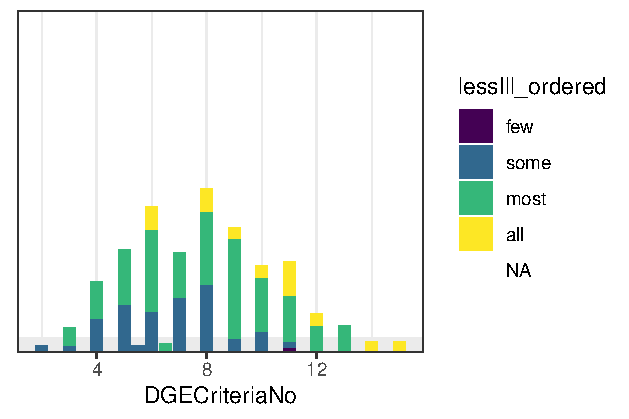
\includegraphics[width=\maxwidth]{figure/beamer-lessIllDGEplot-1} 

}



\end{knitrout}
\end{frame}

\begin{frame}[fragile]
\frametitle{Variable \glqq erweitertes Ernährungswissen\grqq: Zusammenhang mit DGE-Kriterium}
\begin{knitrout}\footnotesize
\definecolor{shadecolor}{rgb}{0.969, 0.969, 0.969}\color{fgcolor}

{\centering 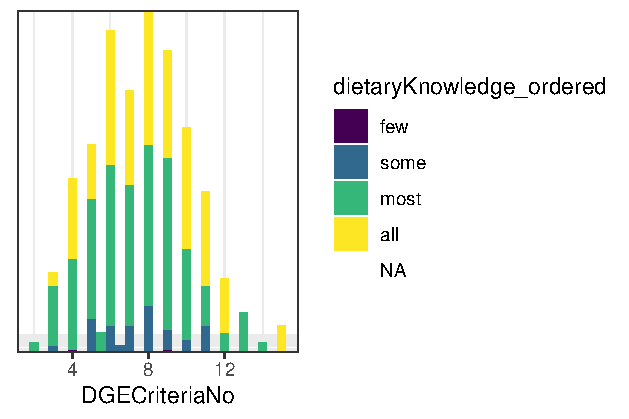
\includegraphics[width=\maxwidth]{figure/beamer-dietaryDGEplot-1} 

}



\end{knitrout}
\end{frame}

\begin{frame}[fragile]
\frametitle{Variable \glqq Wertschätzung gesunder Ernährung\grqq: Zusammenhang mit DGE-Kriterium}
\begin{knitrout}\footnotesize
\definecolor{shadecolor}{rgb}{0.969, 0.969, 0.969}\color{fgcolor}

{\centering 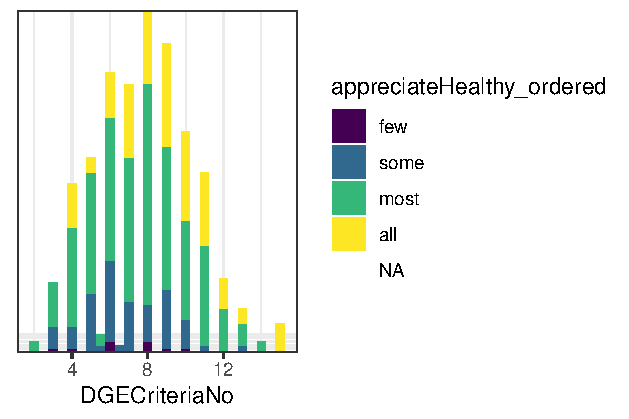
\includegraphics[width=\maxwidth]{figure/beamer-appreciateDGEplot-1} 

}



\end{knitrout}
\end{frame}

\begin{frame}[fragile]
\frametitle{Variable \glqq seltener krank\grqq: Zusammenhang mit DGE-Kriterium}

\begin{table}
\caption{Zusammenhang zwischen DGE-Kriterium und Variable 'seltener krank'}
\begin{center}
\scalebox{0.65}{
\begin{tabular}{l c c c c c }
\hline
 & (1) & (2) & (3) & (4) & (5) \\
\hline
(Intercept)         & $0.02$       & $0.46^{**}$ & $0.09$       & $0.39^{***}$ & $0.05$       \\
                    & $(0.08)$     & $(0.16)$    & $(0.07)$     & $(0.12)$     & $(0.07)$     \\
DGECriteriaNoScaled & $0.33^{***}$ & $0.35^{*}$  & $0.25^{***}$ & $0.24$       & $0.18^{*}$   \\
                    & $(0.08)$     & $(0.16)$    & $(0.07)$     & $(0.14)$     & $(0.07)$     \\
ML1                 &              &             &              &              & $0.12^{*}$   \\
                    &              &             &              &              & $(0.06)$     \\
ML2                 &              &             &              &              & $0.27^{***}$ \\
                    &              &             &              &              & $(0.06)$     \\
\hline
R$^2$               & 0.12         & 0.29        & 0.07         & 0.16         & 0.19         \\
Adj. R$^2$          & 0.11         & 0.29        & 0.07         & 0.16         & 0.17         \\
Num. obs.           & 121          & 120         & 177          & 177          & 161          \\
RMSE                & 0.91         & 7.83        & 0.94         & 7.95         & 0.87         \\
\hline
\multicolumn{6}{l}{\scriptsize{\parbox{\linewidth}
{\vspace{2pt} Dependent variable: share of beneficiaries who are less frequently ill \\ DGECriteriaNo: index of healthy diet criteria fulfilled in organization's menu \\ Model (1): original data set, simple linear model, estimated with OLS \\ Model (2): original data set, simple linear model, estimated with WLS \\ Model (3): imputed data set, simple linear model, estimated with OLS \\ Model (4): imputed data set, simple linear model, estimated with WLS \\ Model (5): imputed data set, linear model with extracted factor scores as controls, estimated with OLS \\ All regressions are estimated with robust standard errors $^{***}p<0.001$, $^{**}p<0.01$, $^*p<0.05$.}}}
\end{tabular}
}
\label{HealthRegressions-LessIll}
\end{center}
\end{table}

\end{frame}

\begin{frame}
\frametitle{Variable \glqq erweitertes Ernährungswissen\grqq: Zusammenhang mit DGE-Kriterium}

\begin{table}
\caption{Zusammenhang zwischen DGE-Kriterium und Variable 'erweitertes Ernährungswissen'}
\begin{center}
\scalebox{0.55}{
\begin{tabular}{l c c c c c }
\hline
 & (1) & (2) & (3) & (4) & (5) \\
\hline
(Intercept)         & $0.02$   & $0.08$   & $0.02$     & $0.21$   & $0.02$       \\
                    & $(0.07)$ & $(0.19)$ & $(0.06)$   & $(0.18)$ & $(0.07)$     \\
DGECriteriaNoScaled & $0.11$   & $-0.02$  & $0.12^{*}$ & $0.10$   & $-0.00$      \\
                    & $(0.06)$ & $(0.12)$ & $(0.05)$   & $(0.14)$ & $(0.06)$     \\
ML1                 &          &          &            &          & $0.26^{***}$ \\
                    &          &          &            &          & $(0.06)$     \\
ML2                 &          &          &            &          & $0.24^{***}$ \\
                    &          &          &            &          & $(0.06)$     \\
ML3                 &          &          &            &          & $0.37^{***}$ \\
                    &          &          &            &          & $(0.06)$     \\
\hline
R$^2$               & 0.01     & 0.00     & 0.02       & 0.01     & 0.31         \\
Adj. R$^2$          & 0.01     & -0.00    & 0.01       & 0.01     & 0.29         \\
Num. obs.           & 214      & 212      & 275        & 275      & 161          \\
RMSE                & 0.98     & 8.49     & 0.96       & 9.45     & 0.83         \\
\hline
\multicolumn{6}{l}{\scriptsize{\parbox{\linewidth}
{\vspace{2pt} Dependent variable: share of beneficiaries with expanded dietary knowledge \\ DGECriteriaNo: index of healthy diet criteria fulfilled in organization's menu \\ Model (1): original data set, simple linear model, estimated with OLS \\ Model (2): original data set, simple linear model, estimated with WLS \\ Model (3): imputed data set, simple linear model, estimated with OLS \\ Model (4): imputed data set, simple linear model, estimated with WLS \\ Model (5): imputed data set, linear model with extracted factor scores as controls, estimated with OLS \\ All regressions are estimated with robust standard errors $^{***}p<0.001$, $^{**}p<0.01$, $^*p<0.05$.}}}
\end{tabular}
}
\label{HealthRegressions-DietaryKnowledge}
\end{center}
\end{table}

\end{frame}

\begin{frame}[fragile]
\frametitle{Variable \glqq Wertschätzung gesunder Ernährung\grqq: Zusammenhang mit DGE-Kriterium}

\begin{table}
\caption{Zusammenhang zwischen DGE-Kriterium und Variable 'Wertschätzung gesunder Ernährung'}
\begin{center}
\scalebox{0.5}{
\begin{tabular}{l c c c c c }
\hline
 & (1) & (2) & (3) & (4) & (5) \\
\hline
(Intercept)         & $-0.03$      & $0.26$   & $0.02$       & $0.37^{*}$ & $0.05$       \\
                    & $(0.07)$     & $(0.18)$ & $(0.06)$     & $(0.17)$   & $(0.07)$     \\
DGECriteriaNoScaled & $0.27^{***}$ & $-0.02$  & $0.25^{***}$ & $0.01$     & $0.03$       \\
                    & $(0.07)$     & $(0.15)$ & $(0.06)$     & $(0.13)$   & $(0.06)$     \\
ML1                 &              &          &              &            & $0.03$       \\
                    &              &          &              &            & $(0.07)$     \\
ML2                 &              &          &              &            & $0.47^{***}$ \\
                    &              &          &              &            & $(0.05)$     \\
ML3                 &              &          &              &            & $0.24^{***}$ \\
                    &              &          &              &            & $(0.05)$     \\
\hline
R$^2$               & 0.06         & 0.00     & 0.06         & 0.00       & 0.37         \\
Adj. R$^2$          & 0.06         & -0.00    & 0.06         & -0.00      & 0.35         \\
Num. obs.           & 213          & 211      & 274          & 274        & 161          \\
RMSE                & 1.02         & 8.61     & 1.01         & 9.00       & 0.82         \\
\hline
\multicolumn{6}{l}{\scriptsize{\parbox{\linewidth}
{\vspace{2pt} Dependent variable: share of beneficiaries with increased appreciation for a healthy diet \\ DGECriteriaNo: index of healthy diet criteria fulfilled in organization's menu \\ Model (1): original data set, simple linear model, estimated with OLS \\ Model (2): original data set, simple linear model, estimated with WLS \\ Model (3): imputed data set, simple linear model, estimated with OLS \\ Model (4): imputed data set, simple linear model, estimated with WLS \\ Model (5): imputed data set, linear model with extracted factor scores as controls, estimated with OLS \\ All regressions are estimated with robust standard errors $^{***}p<0.001$, $^{**}p<0.01$, $^*p<0.05$.}}}
\end{tabular}
}
\label{HealthRegressions-AppreciateHealthy}
\end{center}
\end{table}

\end{frame}

\begin{frame}
\frametitle{Zusammenfassung der Ergebnisse}


\begin{itemize}
\item Einfaches lineares Modell, geschätzt mit OLS: Großer, teilweise signifikanter Zusammenhang zwischen DGE-Kriterium und gesundheitsrelevanten Variablen 
\item Hinzunahme von extrahierten Faktoren als Kontrollen:
\begin{itemize}

\item Variable \glqq seltener krank\grqq: nach wie vor großer, statistisch signifikanter Koeffizient
\item Variablen \glqq erweitertes Ernährungswissen\grqq und \glqq Wertschätzung gesunder Ernährung\grqq: kein Zusammenhang mehr erkennbar
\end{itemize}
\end{itemize}
\end{frame}


\section{Effekte des Entdeckerfonds}

\subsection{Idee}

\begin{frame}[fragile]
\frametitle{Fragestellung}
\begin{itemize}
\item Welchen Effekt besitzt die Förderung einer sozialen Einrichtung durch den CHILDREN Entdeckerfonds auf die teilnehmenden Kinder und Jugendlichen?
\item Herausforderung: Identifizieren einer geeigneten empirischen Methode, um die Wirkungseffekte des CHILDREN Entdeckerfonds zu bestimmen
\linebreak
\item Hypothese: Die Teilnahme einer sozialen Einrichtung am CHILDREN Entdeckerfonds besitzt einen positiven Effekt auf die Alltagskompetenzen und das Selbstwertgefühl der Kinder und Jugendlichen
\end{itemize}
\end{frame}


\begin{frame}[fragile]
\frametitle{Hintergrund}
\begin{itemize}
\item Alle geförderten Einrichtungen erhalten finanzielle Mittel für die Bereitstellung des CHILDREN Mittagstischs
\item Aber: Nicht jede soziale Einrichtung nimmt am CHILDREN Entdeckerfonds teil, um den Kindern und Jugendlichen Ausflüge und Aktivitäten anzubieten
\linebreak
\item [$\Rightarrow$] Der Unterschied zwischen den Einrichtungen hinsichtlich der Teilnahme am CHILDREN Entdeckerfonds wird dazu verwendet, um die Wirkung des Programms zu messen
\end{itemize}
\end{frame}

\subsection{Empirische Methode}

\begin{frame}[fragile]
\frametitle{Einteilung in Treatment- und Kontrollgruppe}
\begin{itemize}
\item Treatmentgruppe: Alle Einrichtungen, die sowohl am CHILDREN Mittagstisch als auch am CHILDREN Entdeckerfonds teilnehmen
\item Kontrollgruppe: Alle Einrichtungen, die nicht am CHILDREN Entdeckerfonds teilnehmen, sondern nur durch den CHILDREN Mittagstisch gefördert werden
\item Um die Einrichtungen in Treatment- und Kontrollgruppe einzuteilen, wurde analysiert, ob bei den Survey-Fragen zum Entdeckerfonds in einem bestimmten Jahr Angaben gemacht wurden
\end{itemize}
\end{frame}

\begin{frame}[fragile]
\frametitle{Treatment-Variable}
\begin{itemize}
\item Um die Einrichtungen in Treatment- und Kontrollgruppe einzuteilen, wird eine Dummy-Variable konstruiert
\item $TreatEF_{it}$ = 1, wenn Einrichtung $i$ im Jahr $t$ am Entdeckerfonds teilgenommen hat und sich somit in der Treatmentgruppe befindet
\item $TreatEF_{it}$ = 0, wenn Einrichtung $i$ im Jahr $t$ nicht am Entdeckerfonds teilgenommen hat und sich somit in der Kontrollgruppe befindet
\item Die Kontrollgruppe ist wesentlich kleiner als die Treatmentgruppe
\end{itemize}
\end{frame}

\begin{frame}[fragile]
\frametitle{Variante 1}
\begin{itemize}
\item \glqq Einmal Treatment, immer Treatment\grqq
\item Sobald eine Einrichtung am Entdeckerfonds teilgenommen hat, gilt $TreatEF_{it}$ = 1 für das Jahr der ersten Förderung durch den Entdeckerfonds und alle darauffolgenden Jahre
\item [$\Rightarrow$] Kein Wechsel von der Treatmentgruppe in die Kontrollgruppe möglich
\item Solange eine Einrichtung keine Förderung vom CHILDREN Entdeckerfonds erhält, befindet sich diese in der Kontrollgruppe
\end{itemize}
\end{frame}

\begin{frame}[fragile]
\frametitle{Variante 2}
\begin{itemize}
\item Zeit-flexibler Treatment-Dummy
\item Eine Einrichtung befindet sich im Jahr $t$ nur dann in der Treatmentgruppe, wenn diese tatsächlich Fördergelder vom CHILDREN Entdeckerfonds erhalten hat
\item [$\Rightarrow$] Wechsel von der Treatmentgruppe in die Kontrollgruppe möglich
\end{itemize}
\end{frame}

\begin{frame}[fragile]
\frametitle{Zielvariable}
\begin{itemize}
\item Problem: Keine Variablen zum Entdeckerfonds für Einrichtungen, die nicht am Entdeckerfonds teilgenommen haben (= Kontrollgruppe) 
\item Verwendete Zielvariablen vom Mittagstisch: Alltagskompetenzen und Selbstwertgefühl
\item [$\Rightarrow$] Anwendbar auf den CHILDREN Mittagstisch und den CHILDREN Entdeckerfonds 
\item [$\Rightarrow$] Über den gesamten Beobachtungszeitraum verfügbar
\item [$\Rightarrow$] Die Alltagskompetenzen und das Selbstwertgefühl der Kinder und Jugendlichen könnten dadurch beeinflusst werden, dass eine Einrichtung am Entdeckerfonds teilnimmt
\end{itemize}
\end{frame}

\begin{frame}[fragile]
\frametitle{Graphische Darstellung: Alltagskompetenzen}
\begin{knitrout}\footnotesize
\definecolor{shadecolor}{rgb}{0.969, 0.969, 0.969}\color{fgcolor}

{\centering 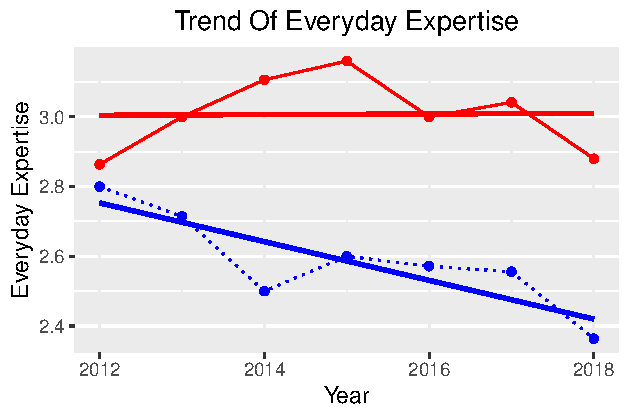
\includegraphics[width=\maxwidth]{figure/beamer-DIDDtdsplot-1} 

}



\end{knitrout}
\end{frame}

\begin{frame}[fragile]
\frametitle{Graphische Darstellung: Selbstwertgefühl}
\begin{knitrout}\footnotesize
\definecolor{shadecolor}{rgb}{0.969, 0.969, 0.969}\color{fgcolor}

{\centering 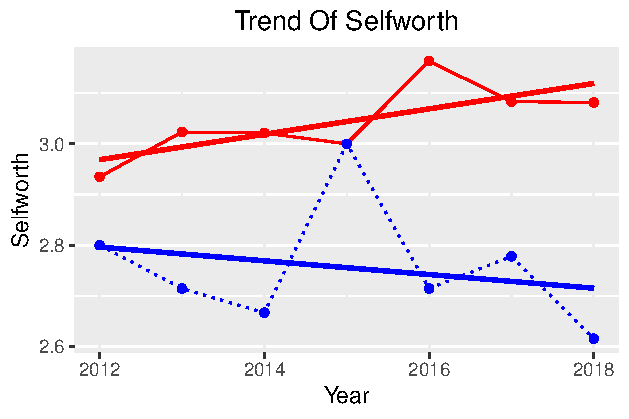
\includegraphics[width=\maxwidth]{figure/beamer-DIDSelfworthplot-1} 

}



\end{knitrout}
\end{frame}

\begin{frame}[fragile]
\frametitle{DID - Schätzung}
\begin{itemize}
\item Empirische Methode: Differences-in-Differences (DID)
\item Der DID-Schätzer misst den Effekt des Entdeckerfonds, indem die Veränderung der abhängigen Variable über die Zeit in der Treatmentgruppe mit der Veränderung in der Kontrollgruppe verglichen wird
\linebreak
\item Regressionsgleichung:
\end{itemize}

\begin{equation}
\label{DID equation}
  Y_{it} = \alpha + \beta \cdot TreatEF_{it} + \gamma_{i} + \delta_{t} + \epsilon_{it}
\end{equation}

\begin{itemize}
\item $\gamma_{i}$ = Einrichtungs-Fixed Effects, $\delta_{t}$ = Jahr-Fixed Effects
\item Der Regressionskoeffizient $\beta$ entspricht dem DID-Schätzer
\end{itemize}
\end{frame}

\begin{frame}[fragile]
\frametitle{Annahmen und Probleme}
\begin{itemize}
\item[ ] Zentrale Annahme des DID-Ansatzes:
\item Commond Trend Assumption: Ohne den Entdeckerfonds würden sich die Zielvariablen in der Treatment- und Kontrollgruppe mit dem gleichen Trend entwickeln
\linebreak
\item[ ] Potentielle Probleme:
\item Verletzung der Common Trend Assumption
\item Selection bias / Endogenität: Nicht zufällig, welche Einrichtungen am Entdeckerfonds teilnehmen
\item [$\Rightarrow$] Implementierung von Kontrollvariablen, die sich auf die Eigenschaften der geförderten Einrichtungen beziehen
\end{itemize}
\end{frame}

\subsection{Ergebnisse}

\begin{frame}[fragile]
\frametitle{Alltagskompetenzen}
\begin{table}
\begin{center}
\scalebox{0.8}{
\begin{tabular}{l c c c c }
\\[-1.8ex]\hline
& \multicolumn{4}{c}{\textit{Abhängige Variable:}} \\
\cline{2-5}
\\[-1.8ex] & \multicolumn{4}{c}{Alltagskompetenzen} \\
\hline
 & (1) & (2) & (3) & (4) \\
\hline
treatEF     & $-0.143$  & $-0.166$     & $0.247$   & $0.255$      \\
            & $(0.402)$ & $(0.405)$    & $(0.299)$ & $(0.310)$    \\
subsidy     &           & $0.019$      &           & $0.016$      \\
            &           & $(0.014)$    &           & $(0.014)$    \\
totalCost   &           & $0.001^{**}$ &           & $0.001^{*}$  \\
            &           & $(0.000)$    &           & $(0.000)$    \\
weeklyCooks &           & $0.166^{**}$ &           & $0.162^{**}$ \\
            &           & $(0.072)$    &           & $(0.073)$    \\
\hline
ID fixed effects       & $Yes$     & $Yes$        & $Yes$     & $Yes$        \\
Year fixed effects     & $Yes$     & $Yes$        & $Yes$     & $Yes$        \\
Number of observations & $428$     & $410$        & $428$     & $410$        \\
R$^2$                  & $0.475$   & $0.490$      & $0.476$   & $0.491$      \\
\hline
\multicolumn{5}{l}{\scriptsize{$^{***}p<0.01$, $^{**}p<0.05$, $^*p<0.1$}}
\end{tabular}
}
\end{center}
\caption{DID-Schätzung: Ergebnisse für Alltagskompetenzen}
\end{table}
\end{frame}

\begin{frame}[fragile]
\frametitle{Alltagskompetenzen}
\begin{itemize}
\item Das Vorzeichen des Effekts hängt von der Definition der Treatment-Variable ab
\item Hauptresultat: Die Teilnahme einer Einrichtung am Entdeckerfonds besitzt keinen statistisch signifikanten Effekt auf die Alltagskompetenzen der Kinder und Jugendlichen
\item Aber: Die Anzahl der Beobachtungseinheiten in der Kontrollgruppe ist sehr gering
\item Wenn der Stichprobenumfang steigt, dann könnte der Effekt des Entdeckerfonds gegebenenfalls positiv und statistisch signifikant werden
\end{itemize}
\end{frame}

\begin{frame}[fragile]
\frametitle{Selbstwertgefühl}
\begin{table}
\begin{center}
\scalebox{0.8}{
\begin{tabular}{l c c c c }
\\[-1.8ex]\hline
& \multicolumn{4}{c}{\textit{Abhängige Variable:}} \\
\cline{2-5}
\\[-1.8ex] & \multicolumn{4}{c}{Selbstwertgefühl} \\
\hline
 & (1) & (2) & (3) & (4) \\
\hline
treatEF     & $-0.474$  & $-0.481$  & $-0.328$  & $-0.442^{*}$ \\
            & $(0.309)$ & $(0.312)$ & $(0.247)$ & $(0.256)$    \\
subsidy     &           & $0.011$   &           & $0.014$      \\
            &           & $(0.018)$ &           & $(0.017)$    \\
totalCost   &           & $0.000$   &           & $0.000$      \\
            &           & $(0.001)$ &           & $(0.001)$    \\
weeklyCooks &           & $0.036$   &           & $0.037$      \\
            &           & $(0.069)$ &           & $(0.069)$    \\
\hline
ID fixed effects       & $Yes$     & $Yes$     & $Yes$     & $Yes$        \\
Year fixed effects     & $Yes$     & $Yes$     & $Yes$     & $Yes$        \\
Number of observations & $428$     & $410$     & $428$     & $410$        \\
R$^2$                  & $0.475$   & $0.484$   & $0.474$   & $0.485$      \\
\hline
\multicolumn{5}{l}{\scriptsize{$^{***}p<0.01$, $^{**}p<0.05$, $^*p<0.1$}}
\end{tabular}
}
\caption{DID-Schätzung: Ergebnisse für Selbstwertgefühl}
\end{center}
\end{table}
\end{frame}

\begin{frame}[fragile]
\frametitle{Selbstwertgefühl}
\begin{itemize}
\item Hauptresultat: Der Effekt des Entdeckerfonds auf das Selbstwertgefühl der Kinder und Jugendlichen ist negativ und teilweise statistisch signifikant
\linebreak
\item [ ] Mögliche Gründe:
\item Die Anzahl der Beobachtungseinheiten in der Kontrollgruppe ist gering
\item Die Fragenbögen werden nicht direkt von den Kindern und Jugendlichen beantwortet, sondern von den Betreuern der geförderten Einrichtungen
\item Die Skalierung der Zielvariable \glqq Selbstwertgefühl\grqq{} führt zu geringer Variation
\item [$\Rightarrow$] Daher sollte dieses Ergebnis nicht überinterpretiert werden
\end{itemize}
\end{frame}

\begin{frame}
\frametitle{Statistisches Lob für CHILDREN}
\begin{itemize}
\item<1-> Erfassung vieler Variablen über die ganze Zeit
\item<2-> Unveränderte Datenskala (alle bis keine)
\item<3-> Erfassung von zwei Variablen sowohl bei Mittagstisch als auch bei Entdeckerfonds
\item<4-> Fragebogen wird automatisch ausgefüllt $\Rightarrow$ wenige fehlende Werte
\end{itemize}
\end{frame}

\begin{frame}[fragile]
\frametitle{Empfehlungen für CHILDREN}
\begin{itemize}
\item[a)] Datenstruktur und -erhebung:
\item Kinder und Jugendliche direkt befragen
\item Einheitliche Variablen, die jedes Jahr erfragt werden
\item Elektronische Fragebögen und Datenerhebung
\item Ordinale Variablen an sich kein Problem, Ersetzung durch metrische (in Prozent) nur sinnvoll, wenn dadurch nicht häufiger fehlende Werte
\item[b)] Auswahl der Variablen: Ähnliche Variablen durch zugrundeliegende ersetzen, anhand von Faktoranalyse oder Partition 
\item[c)] Interventionen: Noch stärkeres Gewicht auf gesunder Ernährung in Einrichtungen
\end{itemize}
\end{frame}

\frame[allowframebreaks]{\frametitle{References}
		\tiny
		\printbibliography
}

\begin{frame}

Danke für die Zusammenarbeit!

\end{frame}
	
\end{document}


